\documentclass[11.5pt, paper=a4]{article}

\usepackage[utf8]{inputenc}
\usepackage[english]{babel}
\usepackage[T1]{fontenc}

\usepackage{amsmath, amssymb, amscd, amsthm, amsfonts, mathtools}
\usepackage[left=2cm, right=2cm, top=1.5cm]{geometry}

\usepackage{graphicx}
\usepackage{hyperref}
\usepackage{physics}
\usepackage{tikz}
\usepackage{url}
\usepackage[square,numbers]{natbib} \usepackage{tabularx}

\usepackage{braket}
\usepackage{thmtools}
\usepackage{float}

%%% Theorem Style
\theoremstyle{definition}
\newtheorem{theorem}{Theorem}[section]
\newtheorem{definition}[theorem]{Definition}
\newtheorem{lemma}[theorem]{Lemma}
\newtheorem{conjecture}[theorem]{Conjecture}
\newtheorem{corollary}[theorem]{Corollary}

\numberwithin{theorem}{section}

%% Autoref prefixes
\renewcommand{\sectionautorefname}{Section}
\renewcommand{\subsectionautorefname}{Section}
\renewcommand{\subsubsectionautorefname}{Section}
\renewcommand{\figureautorefname}{Figure}
\def\theoremautorefname{Theorem}
\def\lemmaautorefname{Lemma}
\def\definitionautorefname{Definition}
\def\conjectureautorefname{Conjecture}
\def\algorithmautorefname{Algorithm}

%% Writing algorithms

\usepackage{algorithm} % captioning
\usepackage{algpseudocode}

% \def\NoNumber#1{{\def\alglinenumber##1{}\State #1}\addtocounter{ALG@line}{-1}}

\graphicspath{{./Lecture_4/images/}}


\title{Quantum Algorithms, Spring 2022: Lecture 4 Scribe}

\author{Debanil Chowdhury, Rishabh Khanna}

\date{\today}

\begin{document}

\maketitle

\section{Recap of previous lecture}

    \begin{itemize}
        \item Postulates of quantum mechanics.
        \begin{enumerate}
            \item Any isolated physical system is given by its state vector which is a unit vector belonging to a Hilbert Space corresponding to the system’s state space.
            \item Evolution of a closed quantum system is given by a unitary transformation.
            \item To ensure that the evolution maintains the state vector to be a unit vector, the operators preserve trace. Trace preserving operators convert a mutually orthonormal set of vectors to another mutually orthonormal set of vectors.
            \item The state space of a composite physical system is the tensor product of the state spaces of the component systems. There are states in this composite physical system that can not be factorized into states of the individual systems, these states are called entangled states.
            \item Quantum measurements are described by a collection of measurement operators acting on the state space of the system.
        \end{enumerate}
        \item Circuit Model of Quantum Computation
        \begin{enumerate}
            \item Initialization: $\ket{\psi_0} = \ket{0}^{\otimes n}$
            \item Evolution: $\ket{\psi_t} = U_tU_{t-1}\ldots U_1\ket{\psi_0}$
            \item Measurement: Typically we perform measurements in a computational basis.
        \end{enumerate}
        \item A classical computer computes boolean functions with a sequence of logic gates, some of which are universal.
        \item According to Landauer's principle computation has an energy cost.
        \item This motivated the study of reversible computing.
    \end{itemize}

\section{Reversible Computing}
\subsection{Fredkin Gate}
    \begin{itemize}
        \item Output of remaining two bits depends on control bit.
        \item Truth table (C is control bit) -
            \begin{center}
            \begin{tabular}{ |c|c|c|c|c|c| }
            \hline
            C & A & B & C & A' & B'\\
            \hline
            0 & 0 & 0 & 0 & 0 & 0\\
            0 & 0 & 1 & 0 & 0 & 1\\
            0 & 1 & 0 & 0 & 1 & 0\\
            0 & 1 & 1 & 0 & 1 & 1\\
            1 & 0 & 0 & 1 & 0 & 0\\
            1 & 0 & 1 & 1 & 1 & 0\\
            1 & 1 & 0 & 1 & 0 & 1\\
            1 & 1 & 1 & 1 & 1 & 1\\
            \hline
            \end{tabular}
            \end{center}
        \item Fredkin gates are universal
    \end{itemize}
\subsection{CNOT Gate}
    \begin{itemize}
        \item 2 bit input and 2 bit output (Control bit and Target bit).
        \item If C is 0 then T is not flipped. If C is 1 then T is flipped.
        \item Truth table (C is control bit and T is Target bit) -
            \begin{center}
            \begin{tabular}{ |c|c|c|c|c|c| }
            \hline
            C & T & C & T'\\
            \hline
            0 & 0 & 0 & 0\\
            0 & 1 & 0 & 1\\
            1 & 0 & 1 & 1\\
            1 & 1 & 1 & 0\\
            \hline
            \end{tabular}
            \end{center}
        \item Representation -
        \begin{figure}[h]
            \centering
            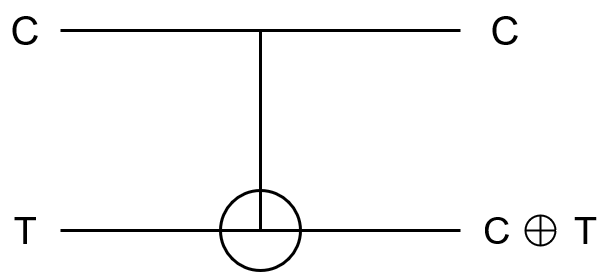
\includegraphics[scale=0.3]{CNOTgate.png}
        \end{figure}
    \end{itemize}
\subsection{Toffoli Gate}
\begin{itemize}
        \item 3 bit input and 3 bit output (2 Control bits and a Target bit).
        \item T is flipped only when both control bits are 1.
        \item Truth table (C is control bit and T is target bit) -
            \begin{center}
            \begin{tabular}{ |c|c|c|c|c|c| }
            \hline
            $C_1$ & $C_2$ & T & $C_1$ & $C_2$ & T'\\
            \hline
            0 & 0 & 0 & 0 & 0 & 0\\
            0 & 0 & 1 & 0 & 0 & 1\\
            0 & 1 & 0 & 0 & 1 & 0\\
            0 & 1 & 1 & 0 & 1 & 1\\
            1 & 0 & 0 & 1 & 0 & 0\\
            1 & 0 & 1 & 1 & 0 & 1\\
            1 & 1 & 0 & 1 & 1 & 1\\
            1 & 1 & 1 & 1 & 1 & 0\\
            \hline
            \end{tabular}
            \end{center}
        \item Representation -
        \begin{figure}[h]
            \centering
            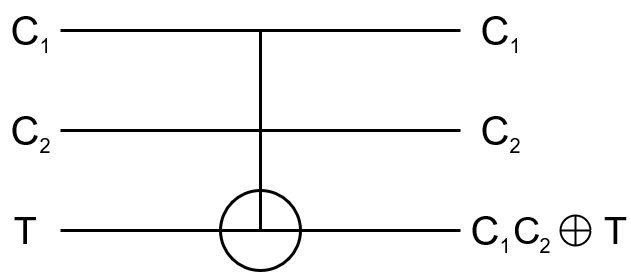
\includegraphics[scale=0.3]{Toffoli.png}
        \end{figure}
    \end{itemize}
\subsection{Garbage bit problem}
\begin{itemize}
    \item Reversible gates have a disadvantage - along with desired output we also get useless garbage output.
    \item In quantum computation, this garbage output can entangle with desired output, hence interfering with computation and producing erroneous result.
    \item Hence in every computation procedure, we should rectify the issue with a procedure called uncomputation that removes garbage output at the expense of some energy dissipation.
\end{itemize}
\subsection{Uncomputation}
\begin{itemize}
    \item Suppose we have a reversible circuit $C_f$ that computes $f$. Lets start with 4 registers.
    \[ (x, 0, 0, y) \longrightarrow (x, f(x), g(x), y) \]
    \item Apply CNOT gate on registers 2 and 4.
    \[ (x, f(x), g(x), y) \longrightarrow (x, f(x), g(x), y \oplus f(x)) \]
    with this we have copied outcome of second register to fourth register.
    \item Apply $C_f^{-1}$. (This is uncomputation).
    \[ (x, f(x), g(x),  y \oplus f(x)) \longrightarrow (x, 0, 0, y \oplus f(x)) \]
    \item This entire process $C_f$, CNOT, $C_f^{-1}$ is typically known as a reversible circuit for $f$.
    \[ (x, y) \longrightarrow (x, y \oplus f(x)) \]
    \item This way, in quantum computing we can uncompute and detangle garbage bits.
\end{itemize}

\newpage
\section{Quantum Gates}
In the circuit model of quantum computing, quantum gates are unitary operators on quantum states. They have to preserve the norm as they map quantum states to other quantum states.
\subsection{Single qubit unitary gates}
\subsubsection{Pauli gates}
    $X = \sigma_{X} = \begin{pmatrix}
    0 & 1\\
    1 & 0
    \end{pmatrix}$
    \begin{figure}[h]
        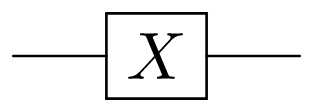
\includegraphics[scale=0.15]{download.png}
    \end{figure}
    $\begin{matrix}
    X\ket{0} = \ket{1}\\
    X\ket{1} = \ket{0}
    \end{matrix}$ \\
    $Y = \sigma_{X} = \begin{pmatrix}
    0 & -i\\
    i & 0
    \end{pmatrix}$ $\begin{matrix}
    Y\ket{0} = i\ket{1}\\
    Y\ket{1} = -i\ket{0}
    \end{matrix}$
    \begin{figure}[h]
        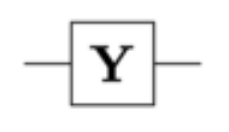
\includegraphics[scale=0.2]{Y gate.png}
    \end{figure} \\
    $Z = \sigma_{X} = \begin{pmatrix}
    1 & 0\\
    0 & -1
    \end{pmatrix}$ $\begin{matrix}
    Z\ket{0} = \ket{0}\\
    Z\ket{1} = -\ket{1}
    \end{matrix}$
    \begin{figure}[h]
        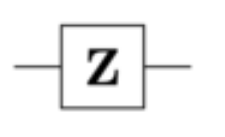
\includegraphics[scale=0.2]{Z gate.png}
    \end{figure}
    \begin{itemize}
        \item $ X^{2} = Y^{2} = Z^{2} = 1 $
    \end{itemize}
\subsubsection{Hadamard gate}
    $Z = \frac{1}{\sqrt{2}}\begin{pmatrix}
    1 & 1\\
    1 & -1
    \end{pmatrix}$ $\begin{matrix}
    H\ket{0} = \frac{1}{\sqrt{2}}(\ket{0} + \ket{1})\\
    H\ket{1} = \frac{1}{\sqrt{2}}(\ket{0} - \ket{1})\\
    \end{matrix}$
\subsubsection{Phase gate}
    $R_{\phi} = \begin{pmatrix}
    1 & 0\\
    0 & e^{i\phi}
    \end{pmatrix}$ $\begin{matrix}
    R_{\phi}\ket{0} = \ket{0} \\
    R_{\phi}\ket{1} = e^{i\phi}\ket{1}
    \end{matrix}$ \\
    $R_{\pi\4} = T\ gate = \begin{pmatrix}
    1 & 0\\
    0 & e^{i\pi/4}
    \end{pmatrix}$ \\
    $R_{\pi\2} = S\ gate = \begin{pmatrix}
    1 & 0\\
    0 & i
    \end{pmatrix}$\\

\begin{itemize}
    \item Pauli matrices give rise to 3 useful unitary matrices when they are exponentialiated (Rotation operations about $\hat{x}$, $\hat{y}$ and $\hat{z}$ axis).\\
        $R_{X}(\theta) = e^{-iX\theta} = cos(\theta)1 - i sin(\theta) X$ \\
        $R_{Y}(\theta) = e^{-iY\theta} = cos(\theta)1 - i sin(\theta) Y$\\
        $R_{Z}(\theta) = e^{-iZ\theta} = cos(\theta)1 - i sin(\theta) Z$ \\
    \newpage

    \item Suppose $\hat{n}$ is a unit vector: $(n_{x}, n_{y}, n_{z})$.   $\hat{\sigma} = (\sigma_{X}, \sigma_{Y}, \sigma_{Z})$\\
    $R_{\hat{n}}(\theta) = e^{-i\hat{n}\hat{\sigma}\theta} = = cos(\theta)1 - i sin(\theta) \hat{n} \hat{\sigma} = cos(\theta)1 - i sin(\theta)(n_{X}\sigma_{X} + n_{y}\sigma_{Y} + n_{Z}\sigma_{Z})$

    \item $U = e^{i\phi}R_{X}(\alpha)R_{Y}(\beta)R_{Z}(\gamma)$

    \item
        \begin{itemize}
            \item Tensor Products: \\
                If gates are applied to different parts of the register.
                \begin{figure}[h]
                    \centering
                    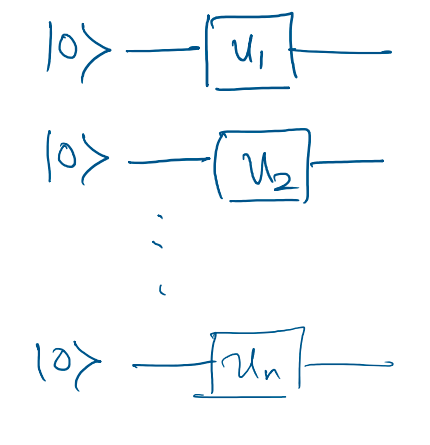
\includegraphics[scale=0.2]{Tensor Product.png}
                \end{figure}\\
                $\ket{\phi} = (U_{1}\otimes U_{2}...\otimes U_{n})\ket{0..0}$\\
                If $\forall j, U_{j}=U$\\
                $\ket{\phi} =   U^{\otimes n}\ket{0..0}$
            \item Ordinary Matrix Products: \\
                If gates are applied sequentially to the same register.
                \begin{figure}[h]
                    \centering
                    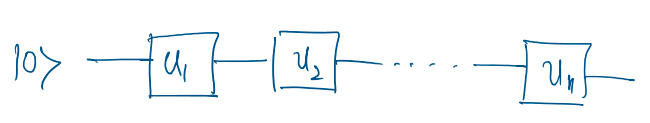
\includegraphics[scale=0.2]{Tensor Product2.png}
                \end{figure}\\
                $\ket{\phi}=U_{n} U_{n-1} ... U_{1}\ket{0}$
        \end{itemize}

    \item Typically a quantum circuit requires both
        \begin{figure}[h]
                    \centering
                    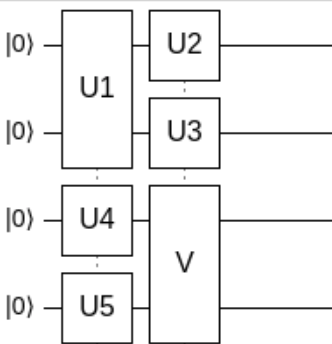
\includegraphics[scale=0.4]{Tensor Product3.png}
                \end{figure}\\

\end{itemize}
\subsubsection{Hadamard gate}
    $H\ket{0} = \frac{1}{\sqrt{2}}(\ket{0} + \ket{1}) = \ket{+}$\\
    $H\ket{1} = \frac{1}{\sqrt{2}}(\ket{0} - \ket{1}) = \ket{-}$\\
    $H\ket{x} = \frac{1}{\sqrt{2}}\sum_{Z \in \{0,1\}}(-1)^{xZ}\ket{Z}$\\ \\
    What about $H_{\otimes n}\ket{0..0}$,
    \begin{align*}
        H_{\otimes n}\ket{0..0} &= \frac{1}{\sqrt{2}}(\ket{0} + \ket{1})\frac{1}{\sqrt{2}}(\ket{0} + \ket{1})..\frac{1}{\sqrt{2}}(\ket{0} + \ket{1}) \\
        &= \frac{1}{\sqrt{2^{n}}}\sum_{j \in \{0, 1\}^{n}}\ket{j}
    \end{align*}
\newpage
\textbf{More Generally:} $\ket{i}=\ket{i_{1}i_{2}..i_{n}}$ and $\ket{j}=\ket{j_{1}j_{2}..j_{n}}$ \\
\begin{align*}
    H^{\otimes n}\ket{i} &= \frac{1}{\sqrt{2^{n}}}*\sum_{j \in \{0,1\}^{n}}(-1)^{i*j}\ket{j} \\
    i*j &= \sum_{k} i_{k} j_{k}
\end{align*}
\begin{align*}
    H^{\otimes n}\ket{i} &= H^{\otimes n}\ket{i_{1} i_{2} .. i_{n}} \\
    &= (H\ket{i_{1}})(H\ket{i_{2}})..(H\ket{i_{n}}) \\
    &= \frac{1}{\sqrt{2^{n}}}* (\sum_{j_{1} \in \{0,1\}}(-1)^{i_{1}j{1}}\ket{j_{1}}) * (\sum_{j_{2} \in \{0,1\}}(-1)^{i_{2}j{2}}\ket{j_{2}}) .. (\sum_{j_{n} \in \{0,1\}}(-1)^{i_{n}j{n}}\ket{j_{n}}) \\
    &= \frac{1}{\sqrt{2^{n}}} \sum_{j_{1}, j_{2} .. j_{n} \in \{0,1\}}(-1)^{i_{1}j_{1} + i_{2}j_{2} .. +i_{n}j_{n}} \ket{j_{1}..j_{n}}\\
    &= \frac{1}{\sqrt{2^{n}}} \sum_{j \in \{0,1\}^{n}} (-1)^{i*j} \ket{j}
\end{align*}
\begin{itemize}
    \item $H^{2} = 1$,
        \begin{align*}
            H^{\otimes n}*H^{\otimes n} &= 1 \\
            &= (H \otimes H \otimes .. H)(H \otimes H \otimes .. H) \\
            &= (H^{2} \otimes H^{2} \otimes .. H^{2}) \\
            &= 1
        \end{align*}
    \item For any unitary circuit $U$ it is easy to find a circuit for $U^{-1}$. It's just $U^{\dagger}$. \\
    $U = U_{1}U_{2}..U_{n}$ then $U^{-1} = U^{\dagger} = U_{n}^{\dagger}U_{n-1}^{\dagger}..U_{1}^{\dagger}$
\end{itemize}
\subsection{2-qubit gates}
\subsubsection{CNOT gate}
$\ket{00} \longmapsto \ket{00}$ \\
$\ket{01} \longmapsto \ket{01}$ \\
$\ket{10} \longmapsto \ket{11}$ \\
$\ket{11} \longmapsto \ket{10}$ \\
$ \hat{U} = \begin{pmatrix}
1 & 0 & 0 & 0 \\
0 & 1 & 0 & 0 \\
0 & 0 & 0 & 1 \\
0 & 0 & 1 & 0 \\
\end{pmatrix} $
\begin{figure}[h]
    \centering
    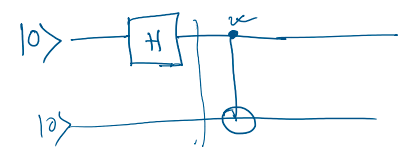
\includegraphics[scale=0.5]{CNOT gate.png}
\end{figure}\\
$\ket{00} \longmapsto^{\hat{H} \otimes 1} (\frac{\ket{0} + \ket{1}}{\sqrt{2}})\ket{0}  \longmapsto^{CNOT} \frac{\ket{00}+\ket{11}}{\sqrt{2}} = \ket{\Phi^{dagger}}$ \\
\newpage
\textbf{Controlled Operations are entangling}
\begin{figure}[h]
    \centering
    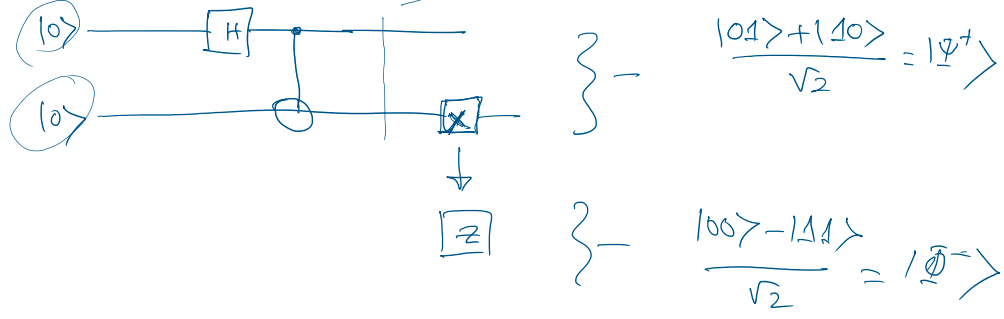
\includegraphics[scale=0.4]{entangling.png}
\end{figure}\\
\subsubsection{SWAP gate}
\begin{itemize}
    \item $S\ket{a,b} = \ket{b,a}$ \\
        \begin{figure}[h]
            \centering
            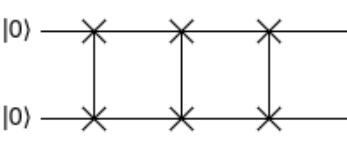
\includegraphics[scale=0.2]{SWAP 3.png}
        \end{figure}\\
        $\ket{a,b} \longmapsto^{CNOT_{a,2}} \ket{a, a,\oplus b} \longmapsto^{CNOT_{2,1}} \ket{a\oplus(a\oplus), a \oplus b} = \ket{b, a \oplus b}$ \\
        $ \ket{b, a \oplus b} \longmapsto^{CNOT_{1,2}} \ket{b, (a\oplusb)\oplusb} = \ket{b, a}$ \\
         \begin{figure}[h]
            \centering
            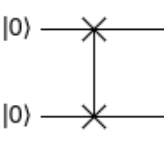
\includegraphics[scale=0.2]{SWAP 1.png}
        \end{figure}\\
\end{itemize}

\end{document}

